\documentclass[11pt,a4paper]{article}

\usepackage{amsfonts}
\usepackage{amssymb}
\usepackage{amsmath}
\usepackage{amsthm}
\usepackage{epsfig}
\usepackage{graphicx}
\usepackage{natbib}		% citet, citep
\usepackage{textcomp}
\usepackage{booktabs}
\usepackage{multirow}
\usepackage{fullpage}
\usepackage{authblk}
\usepackage{url}
\usepackage{color}


\renewcommand{\baselinestretch}{1.4}

\parskip=5pt
\parindent=20pt
\footnotesep=5mm

\newtheorem{lem}{Lemma}
\newtheorem{prop}{Proposition}
\newtheorem{defn}{Definition}
\newtheorem{cor}{Corollary}
\newtheorem{ass}{Assumption}
\newtheorem{obs}{Observation}
\newenvironment{pf}{\begin{proof}\vspace{-10pt}}{\end{proof}}
% \newtheorem{ques}{Question}
% \newtheorem{rmk}{Remark}
% \newtheorem{note}{Note}
% \newtheorem{eg}{Example}

\newenvironment{enumerateTight}{\begin{enumerate}\vspace{-8pt}}{\end{enumerate}\vspace{-8pt}}
\newenvironment{itemizeTight}{\begin{itemize}\vspace{-8pt}}{\end{itemize}\vspace{-8pt}}
\leftmargini=25pt   % default: 25pt
\leftmarginii=12pt  % default: 22pt

\DeclareMathOperator*{\argmax}{argmax}
\DeclareMathOperator*{\argmin}{argmin}






\title{Modeling Product Pricing by Considering 
Consumers' Decisions Based on Utility Maximization}

%\author[1]{Ling-Chieh Kung\thanks{Corresponding author: lckung@ntu.edu.tw}}
%\author[1]{Pei-Yu Sun\thanks{r04725009@ntu.edu.tw}}
%\author[1]{Chien-Yu Huang\thanks{r04725021@ntu.edu.tw}}
%\author[1]{Wei-Che Lee\thanks{r04725023@ntu.edu.tw}}
%\date{\today}
%
%\affil[1]{Department of Information Management, National Taiwan University.}

\author{Ling-Chieh Kung\thanks{Department of Information Management, National Taiwan University; lckung@ntu.edu.tw.}}
\date{}



\begin{document}


%\begin{titlepage}
\maketitle
%\thispagestyle{empty}





%\end{titlepage}







In previous lectures, we have investigated a few game-theoretic models
about a firm's profit maximization problem. 
However, most of these models do not have a role played by consumers. 
In particular, while the firm has a utility function (which is typically 
her profit function or expected profit function) and acts to maximize her 
utility function, the sales outcome is directly assumed to be a function of the 
firm's decision (e.g., $a - bp$ where $p$ is the retail price or 
$\mathbb{E}[\min\{q, D\}]$ where $q$ is the inventory level). 
In this note, we will introduce some models that explicitly models the 
consumers' decisions based on utility maximization. 
In each model, we will see that consumers' have their utility functions, 
and each of them make a decision that maximizes his utility function. 
Being able to model consumers' decisions will enrich our model and 
allow us to tackle more research questions. 







\section{The first model}

Consider the following monopoly pricing problem (which has been introduced 
in the first lecture). A seller sells a product to a market. For consumers 
in the market, their willingness-to-pay $\theta$ uniformly spread within 0 and 1. 
Note that this is saying that consumers are \textit{heterogeneous} on 
their willingness-to-pay for the product. Whenever we have a group of 
heterogeneous consumers, we call the attribute(s) that differentiates 
these consumers their \textit{type}. In this example, 
we call the willingness-to-pay $\theta$ as a consumers' type. 
Let $p$ be the retail price chosen by the seller. 
For the type-$\theta$ consumer, his utility function is 
\[
	u(\theta) = \theta - p 
\]
if he purchases the product and 0 otherwise. 
We say that his \textit{reservation price} is 0. 
Each consumer decides whether to buy the product by considering the product 
price and his own willingness-to-pay $\theta$. 
The unit production cost of the product is $c$. 
The seller chooses $p$ to maximize her profit. 

To solve the seller's problem, we first try to derive the demand function. 
Given a price $p$, a consumer buys the product if and only if his willingness-to-pay
$\theta \geq p$. Therefore, the group of consumers are divided into two 
\textit{segments}: The \textit{high segment} of consumers 
whose $\theta \in [p, 1]$, and the \textit{low segment} of consumers
whose $\theta \in [0, p)$. We sometimes call them \textit{high-end consumers}
and \textit{low-end consumers}, respectively. 
The intuition is clear: One buys the product if and 
only if he sufficiently likes the product. 
The market segmentation then implies that the demand volume is 
\[
	D(p) = 1 - p,
\] 
and the seller's profit-maximization problem is
\[
	\max_p \ (p - c)(1 - p). 
\]
Obviously, the optimal price is $p^* = \frac{1 + c}{2}$. 
The equilibrium profit is $\pi^* = \frac{(1 - c)^2}{4}$. 

Note that we are not assuming the demand function is like this or like that; 
we \textit{derive} the demand function based on our model setting. 
Also note that the assumption of uniformly distributed willingness-to-pay
provides a justification to the widely adopted linear demand setting. 
Finally, note that the consumer of type $p$ is \textit{indifferent} between
buying and not buying. As $\theta$ is continuous, it does not matter 
whether we include him in the high-end or low-end segment. 










\section{Exogenous product quality}

Sometimes we want to model the impact of product quality. 
In particular, may we modify the previous model to include a parameter
$q$ as the product quality so that the equilibrium price and profit will
increase in $q$? 

To do so, let's say the type $\theta$ is now a consumer's willingness-to-pay
\textit{for a unit of quality}. Therefore, the type-$\theta$ consumer's 
utility function becomes
\[
	u(\theta) = \theta q - p
\]
if he purchases a product of quality $q$ and 0 otherwise. 
Note that this setting captures 
three intuitive features. First, one gets happier when the quality becomes higher. 
Second, one gets happier when the price becomes lower. 
Finally, when the quality becomes higher, those of higher $\theta$ 
will have a larger increase than those of lower $\theta$. After all, 
those of higher $\theta$ are willing to pay more for a high quality product, 
so increasing the product quality has a higher impact on them. 
Let's assume that $q$ is exogenous, and the seller may choose $p$ to maximize
her profit. All other settings are the same. 

To solve the seller's problem, again we need to first derive the demand function. 
Given a price $p$, again the market will be divided into two segments (why?), 
and all we need to do is to find the indifferent consumer's type $\theta$. 
In other words, we need to find $\theta_0$ that satisfies
\[
	u(\theta_0) = \theta_0 q - p = 0, 
\]
which implies that $\theta_0 = \frac{p}{q}$. All the consumers whose type 
$\theta \geq \theta_0$ will buy the product (as their utility of buying 
the product is nonnegative) while all others will not. Therefore, 
the high segment is $\theta \in [\frac{p}{q}, 1]$ while the low segment
is $\theta \in [0, \frac{p}{q}]$. 
Therefore, the demand function is 
\[
	D(p) = 1 - \frac{p}{q}, 
\]
and the seller's problem is 
\[
	\max_p \ (p - c)\bigg(1 - \frac{p}{q}\bigg). 
\]
It is still straightforward to solve this problem and obtain the optimal price 
$p^* = \frac{q + c}{2}$. The equilibrium profit is $\pi^* = \frac{(q - c)^2}{4q}$. 
Indeed this model represents the desired fact that both $p^*$ and $\pi^*$ increases
in $q$. 







\section{Endogenous product quality}

What if the product quality $q$ is also a decision variable? 
In this case, typically there should be some cost to increase $q$
(otherwise the seller should always set $q$ to its highest possible value). 
For example, the profit function may become 
\[
	(p - C(q))\bigg(1 - \frac{p}{q}\bigg), 
\]
where the unit production cost $c(q)$ increases in $q$. 
Common choices of $C(q)$ include $cq$ (so the cost is linear to quality)
and $cq^2$ (so the cost is convex to quality) for some $c > 0$.  
Another choice is to consider a profit function
\[
	(p - c)\bigg(1 - \frac{p}{q}\bigg) - C(q). 
\]
In this model, $C(q)$ is the one-time R\&D cost. In any case, 
note that the seller's problem's (joint) concavity needs to be verified. 
Moreover, the problem becomes two-dimensional, i.e. having two decision variables. 
In general more advanced techniques are needed to solve multi-dimensional 
constrained problem. Let's ignore this at this moment. 

An easier model may be obtained by switching from a continuous-type setting 
to a binary-type setting. Instead of letting $\theta$ be uniformly distributed 
between 0 and 1, let $\theta$ follows a Bernoulli distribution of two possible 
values $\theta_L$ and $\theta_H$, where $\theta_L < \theta_H$ and 
\[
	\Pr(\theta = \theta_L) = \beta = 1 - \Pr(\theta = \theta_H).
\]
In other words, we are saying that there are two types of consumers, 
high-end consumers (of type $\theta_H$) and low-end consumers (of type $\theta_L$), 
and the proportion of low-end consumers is $\beta$. 
Let's say the unit production cost is $C(q) = \frac{cq^2}{2}$. 
All other settings are the same. 

To derive the demand function, note that there are only three possible outcomes: 
All consumers buy the product, only high-end consumers buy the product, 
and no consumer buys the product. The seller may adjust $p$ and $q$ to induce
one of these to be the equilibrium outcome. As the last option is obviously not good, 
let's compare the first two strategies. 

To induce all consumers to buy the product, we have 
\[\begin{split}
	\max_{p, q} \quad & 1 \cdot \bigg(p - \frac{cq^2}{2}\bigg) \\
	\mbox{s.t.} \quad & \theta_L q - p \geq 0.
\end{split}\]
The constraint $\theta_L q - p \geq 0$ ensures that all low-end consumers 
are willing to buy the product. Obviously, high-end consumers will also 
buy the product, and thus all consumers will buy the product. 
The demand is then $\beta + (1 - \beta) = 1$. 
For each consumer, the seller earns $p - \frac{cq^2}{2}$. 
To solve this problem, note that the constraint must be binding at 
any optimal solution (otherwise the seller may increase $p$ to make herself better
off). Therefore, for any optimal solution, we have $\theta_L q = p$. 
If we replace $p$ in the objective function by $\theta_L q$, 
we reduce the problem to 
\[
	\max_q \ \theta_L q - \frac{cq^2}{2}. 
\]
The optimal quality level is $q^{\mathrm{all}} = \frac{\theta_L}{c}$. The equilibrium 
profit is $\pi^{\mathrm{all}} = \frac{\theta_L^2}{2c}$. 

Similarly, to induce only the high-end consumers to buy the product, we have 
\[\begin{split}
	\max_{p, q} \quad & (1 - \beta) \bigg(p - \frac{cq^2}{2}\bigg) \\
	\mbox{s.t.} \quad & \theta_H q - p \geq 0.
\end{split}\]
Again, the constraint must be binding at 
any optimal solution, and we may reduce the problem to 
\[
	\max_q \ (1 - \beta) \bigg(\theta_H q - \frac{cq^2}{2}\bigg)
\]
The optimal quality level is $q^{\mathrm{high}} = \frac{\theta_H}{c}$. The equilibrium 
profit is $\pi^{\mathrm{high}} = (1 - \beta)\frac{\theta_H^2}{2c}$. 
Note that when the sellers decides to serve only high-end consumers, 
the optimal product quality gets higher ($q^{\mathrm{high}} > q^{\mathrm{all}}$). 
This is reasonable: As your target consumers are willing to pay more for quality, 
increasing the quality is a good idea. We may verify that the optimal price
is also higher under the high-end-only strategy. 

All the above derivations lead to the following proposition. Figure \ref{fig:strategy} visualizes the result. 

\begin{prop}\label{prop:strategy}
Serving all consumers is better than serving only the high segment if and only if 
\[
	\frac{\theta_L}{\theta_H} > \sqrt{1 - \beta}.
\]
\end{prop}

\begin{figure}[hbt]
\centering
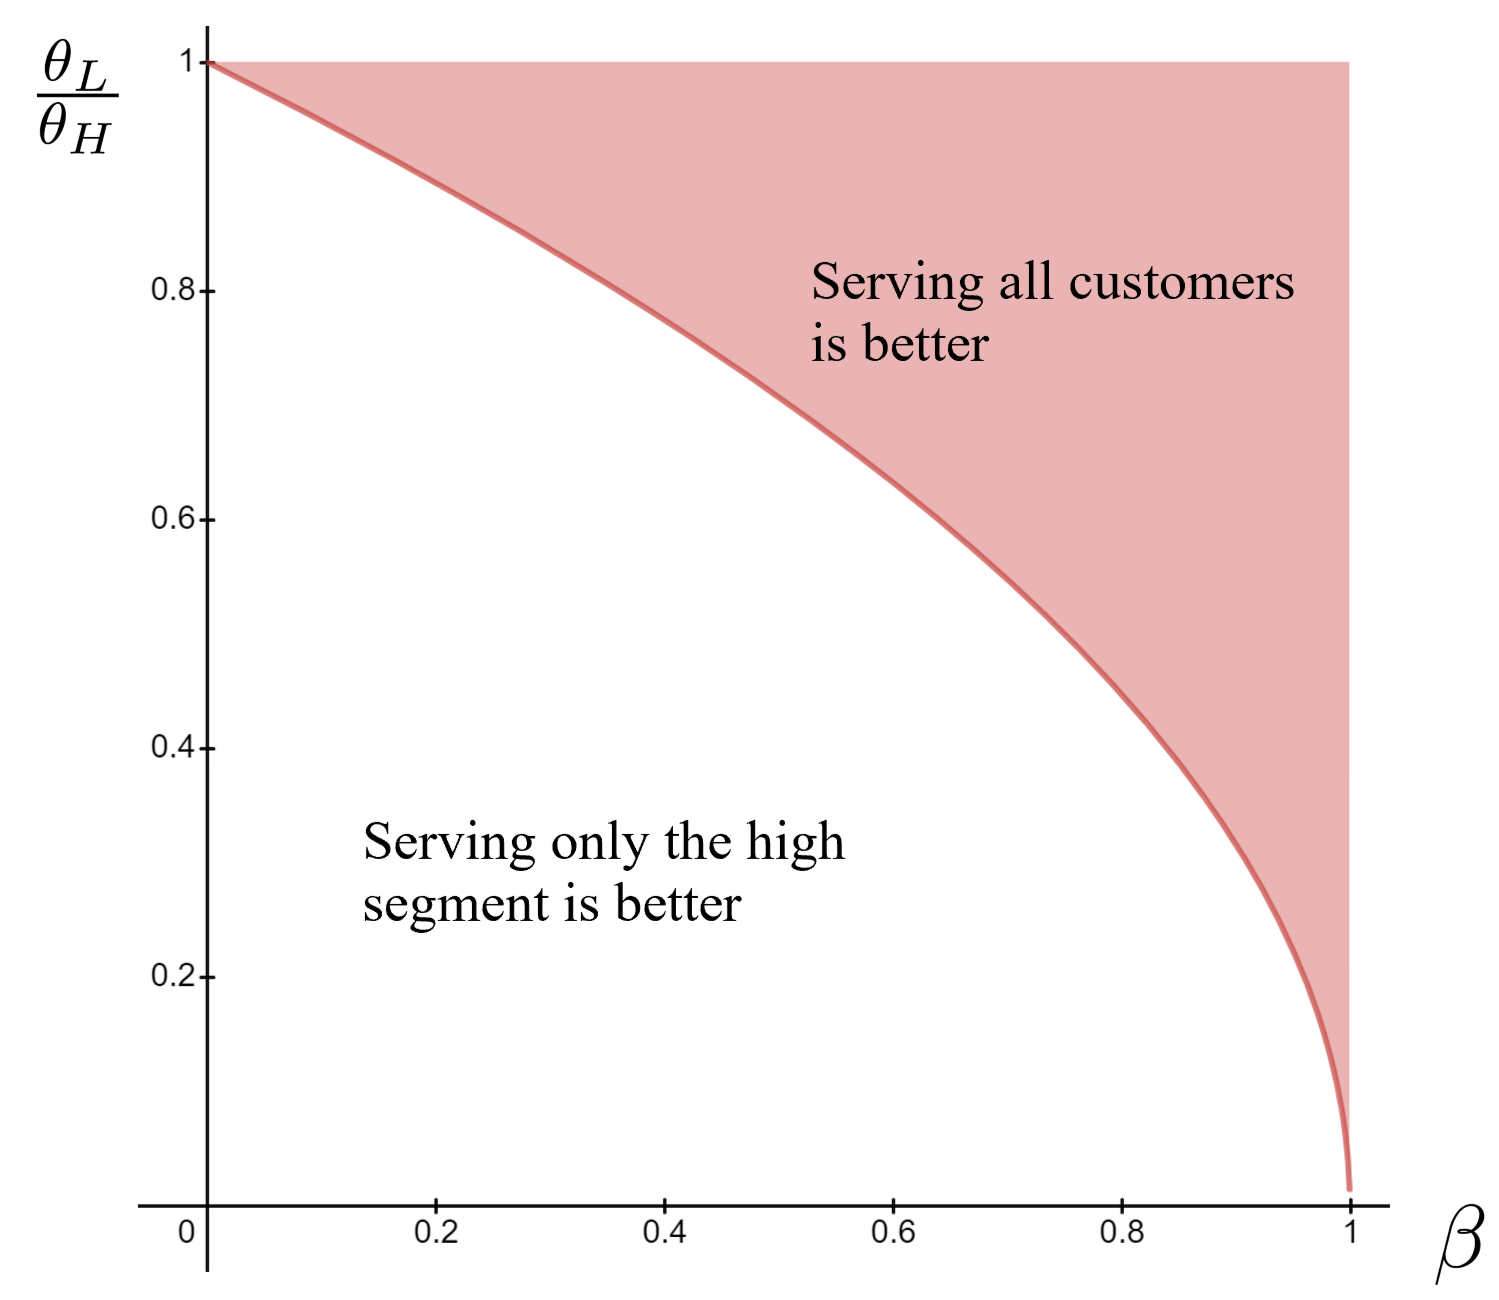
\includegraphics[width=0.5\textwidth]{figures/strategy}
\caption{Strategy choice under endogenous product quality}
\label{fig:strategy}
\end{figure}

According to Proposition \ref{prop:strategy}, what matter are the two willingness-to-pay levels and the relative size of the two groups of consumers. If $\theta_L$ is quite low compared to $\theta_H$, serving the low segment would require the seller to cut down the price by a huge amount. It is then better to serve only the high segment. If $\beta$ is low, which means that the size of low segment is small, it is also the seller's best interest to serve only the high segment. 











\section{Two products}

Let's ignore endogenous quality and go back to the exogenous quality setting. 
What if the seller now has two products, each of quality $q_1$ and $q_2$? 
Without loss of generality, let's assume that $q_1 > q_2$, 
so products 1 and 2 are the high- and low-quality products, respectively. 
The unit production costs of products 1 and 2 are $c_1$ and $c_2$, respectively. 
How to price these two products for profit maximization? 

Given the prices $p_1$ and $p_2$ for products 1 and 2, respectively, 
each consumer has three options: buying product 1, buying product 2, 
or buying nothing. By buying product 1, a type-$\theta$ consumer's utility 
is $\theta q_1 - p_1$. He will be willing to buy product 1 (compared to 
buying nothing) if and only if $\theta \geq \frac{p_1}{q_1}$. 
Similarly, he will be willing to buy product 2 if and only if 
$\theta \geq \frac{p_2}{q_2}$. Now, if a consumer is only willing to buy
one of the two products, he will buy it; if he is willing to buy both, 
he will choose the one that gives him a higher utility. 
In this case, he prefers product 1 if and only if 
\[
	\theta q_1 - p_1 \geq \theta q_2 - p_2 \quad\Leftrightarrow\quad
	\theta \geq \frac{p_1 - p_2}{q_1 - q_2}. 
\]
Let $\theta_1 = \frac{p_1}{q_1}$, $\theta_2 = \frac{p_2}{q_2}$, 
and $\bar{\theta} = \frac{p_1 - p_2}{q_1 - q_2}$, the relationship
among the three cutoff values determines the equilibrium market segmentation. 

Suppose that $\bar{\theta} > \theta_2$, i.e., $p_1q_2 > q_1p_2$. 
In this case, the market will be divided into three segments: 
the high segment $\theta \in [\frac{p_1 - p_2}{q_1 - q_2}, 1]$ of consumers
who buy product 1, 
the middle segment $\theta \in [\frac{p_2}{q_2}, \frac{p_1 - p_2}{q_1 - q_2}]$
of consumers who buy product 2, and 
the low segment $\theta \in [0, \frac{p_2}{q_2}]$ of consumers who buy nothing. 
The seller's profit function is 
\[
	(p_1 - c_1)\bigg(1 - \frac{p_1 - p_2}{q_1 - q_2}\bigg)
	+ (p_2 - c_2)\bigg(\frac{p_1 - p_2}{q_1 - q_2} - \frac{p_2}{q_2}\bigg).
\]
On the contrary, if $\bar{\theta} < \theta_2$, i.e., $p_1q_2 < q_1p_2$,  
the middle segment degenerates and the market will be divided to only two segments: 
the high segment $\theta \in [\frac{p_1}{q_1}, 1]$ of consumers
who buy product 1, and 
the low segment $\theta \in [0, \frac{p_1}{q_1}]$ of consumers who buy nothing. 
The seller's profit function is 
\[
	(p_1 - c_1)\bigg(1 - \frac{p_1}{q_1}\bigg). 
\]

It is the seller's discretion to set $p_1$ and $p_2$ to induce either equilibrium. 
For example, he may set an extremely high $p_2$ to satisfy $p_1 q_2 < q_1 p_2$. 
In this case, no one prefers product 2, and we will have the two-segment equilibrium. 
As the seller's profit function is different under the two market segmentation
strategy, to find the seller's optimal prices, we need to solve two subproblems, 
one for each strategy. In the first subproblem, we solve for $p_1$ and $p_2$ 
under the three-segment equilibrium, i.e, we solve 
\[\begin{split}
	\pi^{\mathrm{three}} = \max_{p_1, p_2} \quad & 
		(p_1 - c_1)\bigg(1 - \frac{p_1 - p_2}{q_1 - q_2}\bigg)
		+ (p_2 - c_2)\bigg(\frac{p_1 - p_2}{q_1 - q_2} - \frac{p_2}{q_2}\bigg) \\
	\mbox{s.t.} \quad & p_1q_2 \geq q_1p_2. 
\end{split}\]
In other words, the seller restricts herself by asking ``if I want to have 
three segments, what are the optimal prices?'' After $\pi^{\mathrm{three}}$ is found, 
the seller should proceed to solve the second subproblem
\[\begin{split}
	\pi^{\mathrm{two}} = \max_{p_1, p_2} \quad & 
		(p_1 - c_1)\bigg(1 - \frac{p_1}{q_1}\bigg) \\
	\mbox{s.t.} \quad & p_1q_2 \leq q_1p_2. 
\end{split}\]
By comparing $\pi^{\mathrm{three}}$ and $\pi^{\mathrm{two}}$, the seller may 
find her optimal strategy. This is called the \textit{product line design} 
problem in the marketing literature. 

Up to now, if you understand the formulation and the concepts of market segmentation
and strategy selection, it is great. Unfortunately, even though the above 
subproblems are not really complicated, we have not taught you in this course 
how to analytically solve these multi-dimensional constrained problems. 
If you really want to solve them, please study the KKT condition by yourself 
or discuss with the instructor. 






\section*{Appendix}

\textbf{Proof of Proposition \ref{prop:strategy}.} 
Serving all consumers is better than serving only the high segment if and only if 
\[
	\pi^{\mathrm{all}} = \frac{\theta_L^2}{2c} 
	> (1 - \beta) \frac{\theta_H^2}{2c} = \pi^{\mathrm{high}}, 
\]
which is equivalent to $\frac{\theta_L}{\theta_H} > \sqrt{1 - \beta}$. \qed





\end{document}
